\documentclass[conference]{IEEEtran}
\IEEEoverridecommandlockouts
% The preceding line is only needed to identify funding in the first footnote. If that is unneeded, please comment it out.
\usepackage{cite}
\usepackage{amsmath,amssymb,amsfonts}
\usepackage{algorithmic}
\usepackage{graphicx}
\usepackage{textcomp}
\usepackage{url}
\usepackage{float}
\usepackage{xcolor}
\def\BibTeX{{\rm B\kern-.05em{\sc i\kern-.025em b}\kern-.08em
    T\kern-.1667em\lower.7ex\hbox{E}\kern-.125emX}}
\begin{document}

\title{Optimized Real-time Cross Traffic Management for Autonomous Vehicles\\
}

\author{\IEEEauthorblockN{1\textsuperscript{st} Rubayet Kamal}
\IEEEauthorblockA{\textit{Electronic Engineering} \\
\textit{Hochschule Hamm-Lippstadt}\\
Lippstadt, Germany \\
rubayet.kamal@stud.hshl.de}
\and
\IEEEauthorblockN{2\textsuperscript{nd} Moiz Zaheer Malik}
\IEEEauthorblockA{\textit{Electronic Engineering} \\
\textit{Hochschule Hamm-Lippstadt}\\
Lippstadt, Germany \\
moiz-zaheer.malik@stud.hshl.de}
\and
\IEEEauthorblockN{3\textsuperscript{rd} Mofifoluwa Akinwande }
\IEEEauthorblockA{\textit{Electronic Engineering} \\
\textit{Hochschule Hamm-Lippstadt}\\
Lippstadt, Germany \\
mofifoluwa-ipadeola.akinwande@stud.hshl.de}
\and
\IEEEauthorblockN{4\textsuperscript{th} Jonathan Bahry}
\IEEEauthorblockA{\textit{Electronic Engineering} \\
\textit{Hochschule Hamm-Lippstadt}\\
Lippstadt, Germany \\
jonathan.bahry@stud.hshl.de}

}

\maketitle

\begin{abstract}
This paper presents a comprehensive technical documentation of a centralized traffic controller for autonomous vehicles designed to manage vehicle crossing through intersections. Motivated by the inefficiencies of traditional traffic light systems and the growing integration of autonomous vehicles. The system employs First-Come, First-Serve (FCFS) queueing model and prioritizes pedestrian safety through sensor based detection. The documentation covers the motivation behind the project, the systems engineering approach, UPAAL for timed automata and behavioral modeling. The software is implemented using FreeRTOS to ensure deterministic task scheduling, and the system is validated through hardware using VHDL. 
\end{abstract}

\begin{IEEEkeywords}
FreeRTOS, FCFS, UPAAL, ModelSim, VHDL
\end{IEEEkeywords}

\section{Introduction and Requirements}
\begin{figure*}[!t]
    \centering
    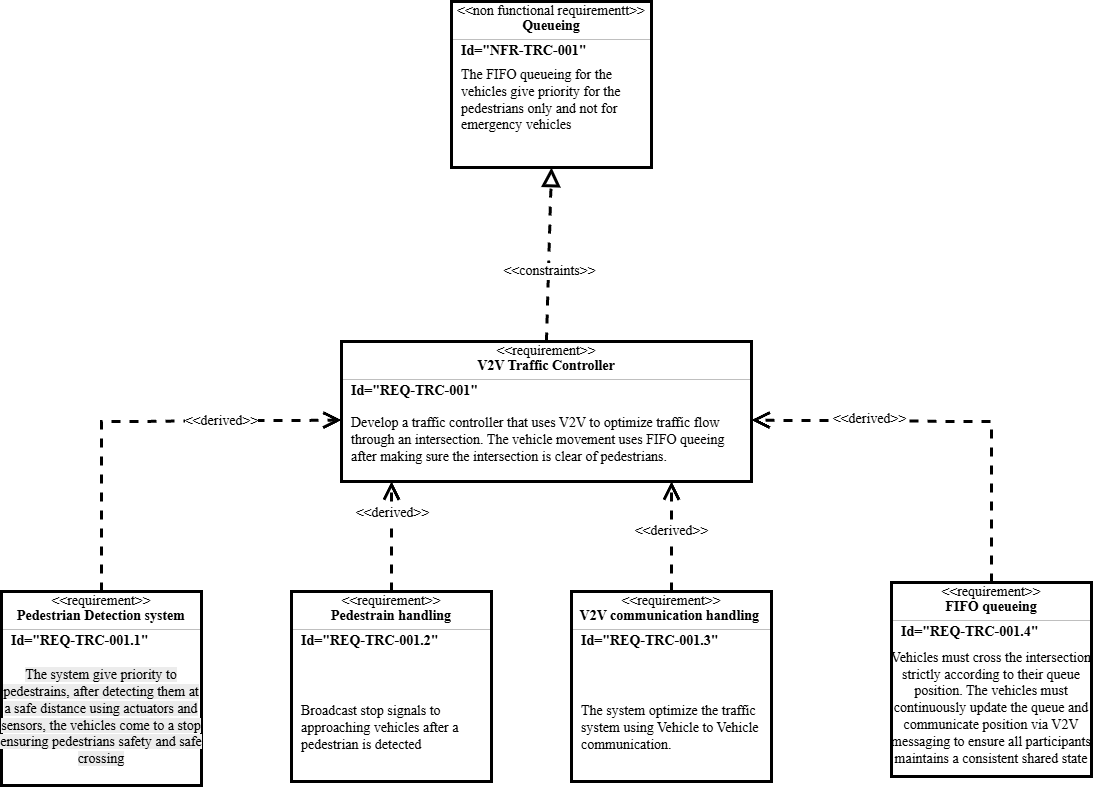
\includegraphics[width=1.0\textwidth]{Pictures/requirement-diagram.png}
    \caption{Requirements Diagram}
    \label{fig:requirements diagram}
\end{figure*}

As cities grow and traffic volumes rise, traditional traffic light systems, while functional, these traffic lights are inefficient and are becoming more insufficient. These systems are leading to reduced flow efficiency, fuel waste and unnecessary delays. Recognizing these limitations, and with the growing relevance of autonomous vehicles.We set out to design an efficient, intelligent traffic control system.

Initially, our approach involved an upgrade or an advanced version of the current traffic light system. Scaling the current system offered some improvements, but it still fell short in addressing the demands of autonomous, coordinated traffic behavior.We then explored a decentralized traffic management approach, relying solely on vehicle-to-vehicle (V2V) communication. Although promising in theory, this concept lacked robustness and consistency leading to many collisions.
Through further research, we identified a new approach, we identified a more effective solution. A centralized traffic controller that communicates directly with the vehicles approaching an intersection. In this system, vehicles broadcasts their intent to cross the intersection, allowing the traffic controller to manage traffic on a First Come First Serve (FCFS) queuing model. Pedestrians are always given priority, ensuring that their right of way is fully respected. This system eliminates the need for traditional traffic light and enables more efficient traffic coordination. 

The development of our traffic controller system was guided by a comprehensive set of requirements, meticulously captured and organized using SysML requirement diagrams. This approach provides a clear visualization of both functional and non functional requirements. At the core of our system lies the fundamental requirement for traffic controller system (REQ-TRC-001). This overarching capability is supported by four primary functional requirements: a pedestrian detection system (REQ-TRC-001.1), pedestrian handling (REQ-TRC-001.2), arbiter communication handling (REQ-TRC-001.3) and FCFS queuing (REQ-TRC-001.4). The pedestrian detection system represents a critical safety feature of our system. This requirement specifies that the system must be able to detect pedestrians at a safe distance giving enough time for the intended vehicles to come to a complete stop. Complementing this, the pedestrian handling requirement ensures that upon the detection of a pedestrian, the system should broadcast this information to all vehicles within the intersection, maintaining situational awareness and ensuring safe crossing. The arbiter communication handling dictates that all communications and decision making is made by the controller itself to avoid the possibility of any collision. The FCFS queuing requirement enforces that vehicles follow a strict FCFS order, continuously updating their queue status and coordinating with the controller to maintain an efficient traffic flow. To ensure the system reliability and performance, we have also included a constraint related to queuing. This stipulates that under all circumstances, the system should fulfill the FCFS queuing even in the presence of emergency vehicles.



\section{Modelling with SysML}
To design and analyze our \textbf{autonomous traffic controller system}, we employed \textbf{Systems Modeling Language (SysML)}. The system is responsible for managing the flow of autonomous vehicles at intersections using a \textbf{first-come, first-served queuing mechanism}, while also accounting for \textbf{pedestrian detection via sensors and actuators}. Communication between the traffic controller and vehicles ensures coordinated movement, with pedestrian presence acting as a high-priority interrupt.

The following SysML diagrams illustrate key behavioral and interaction aspects of the system:

 
\subsection{State Machine Diagram}
\begin{figure*}[t]
    \centering
    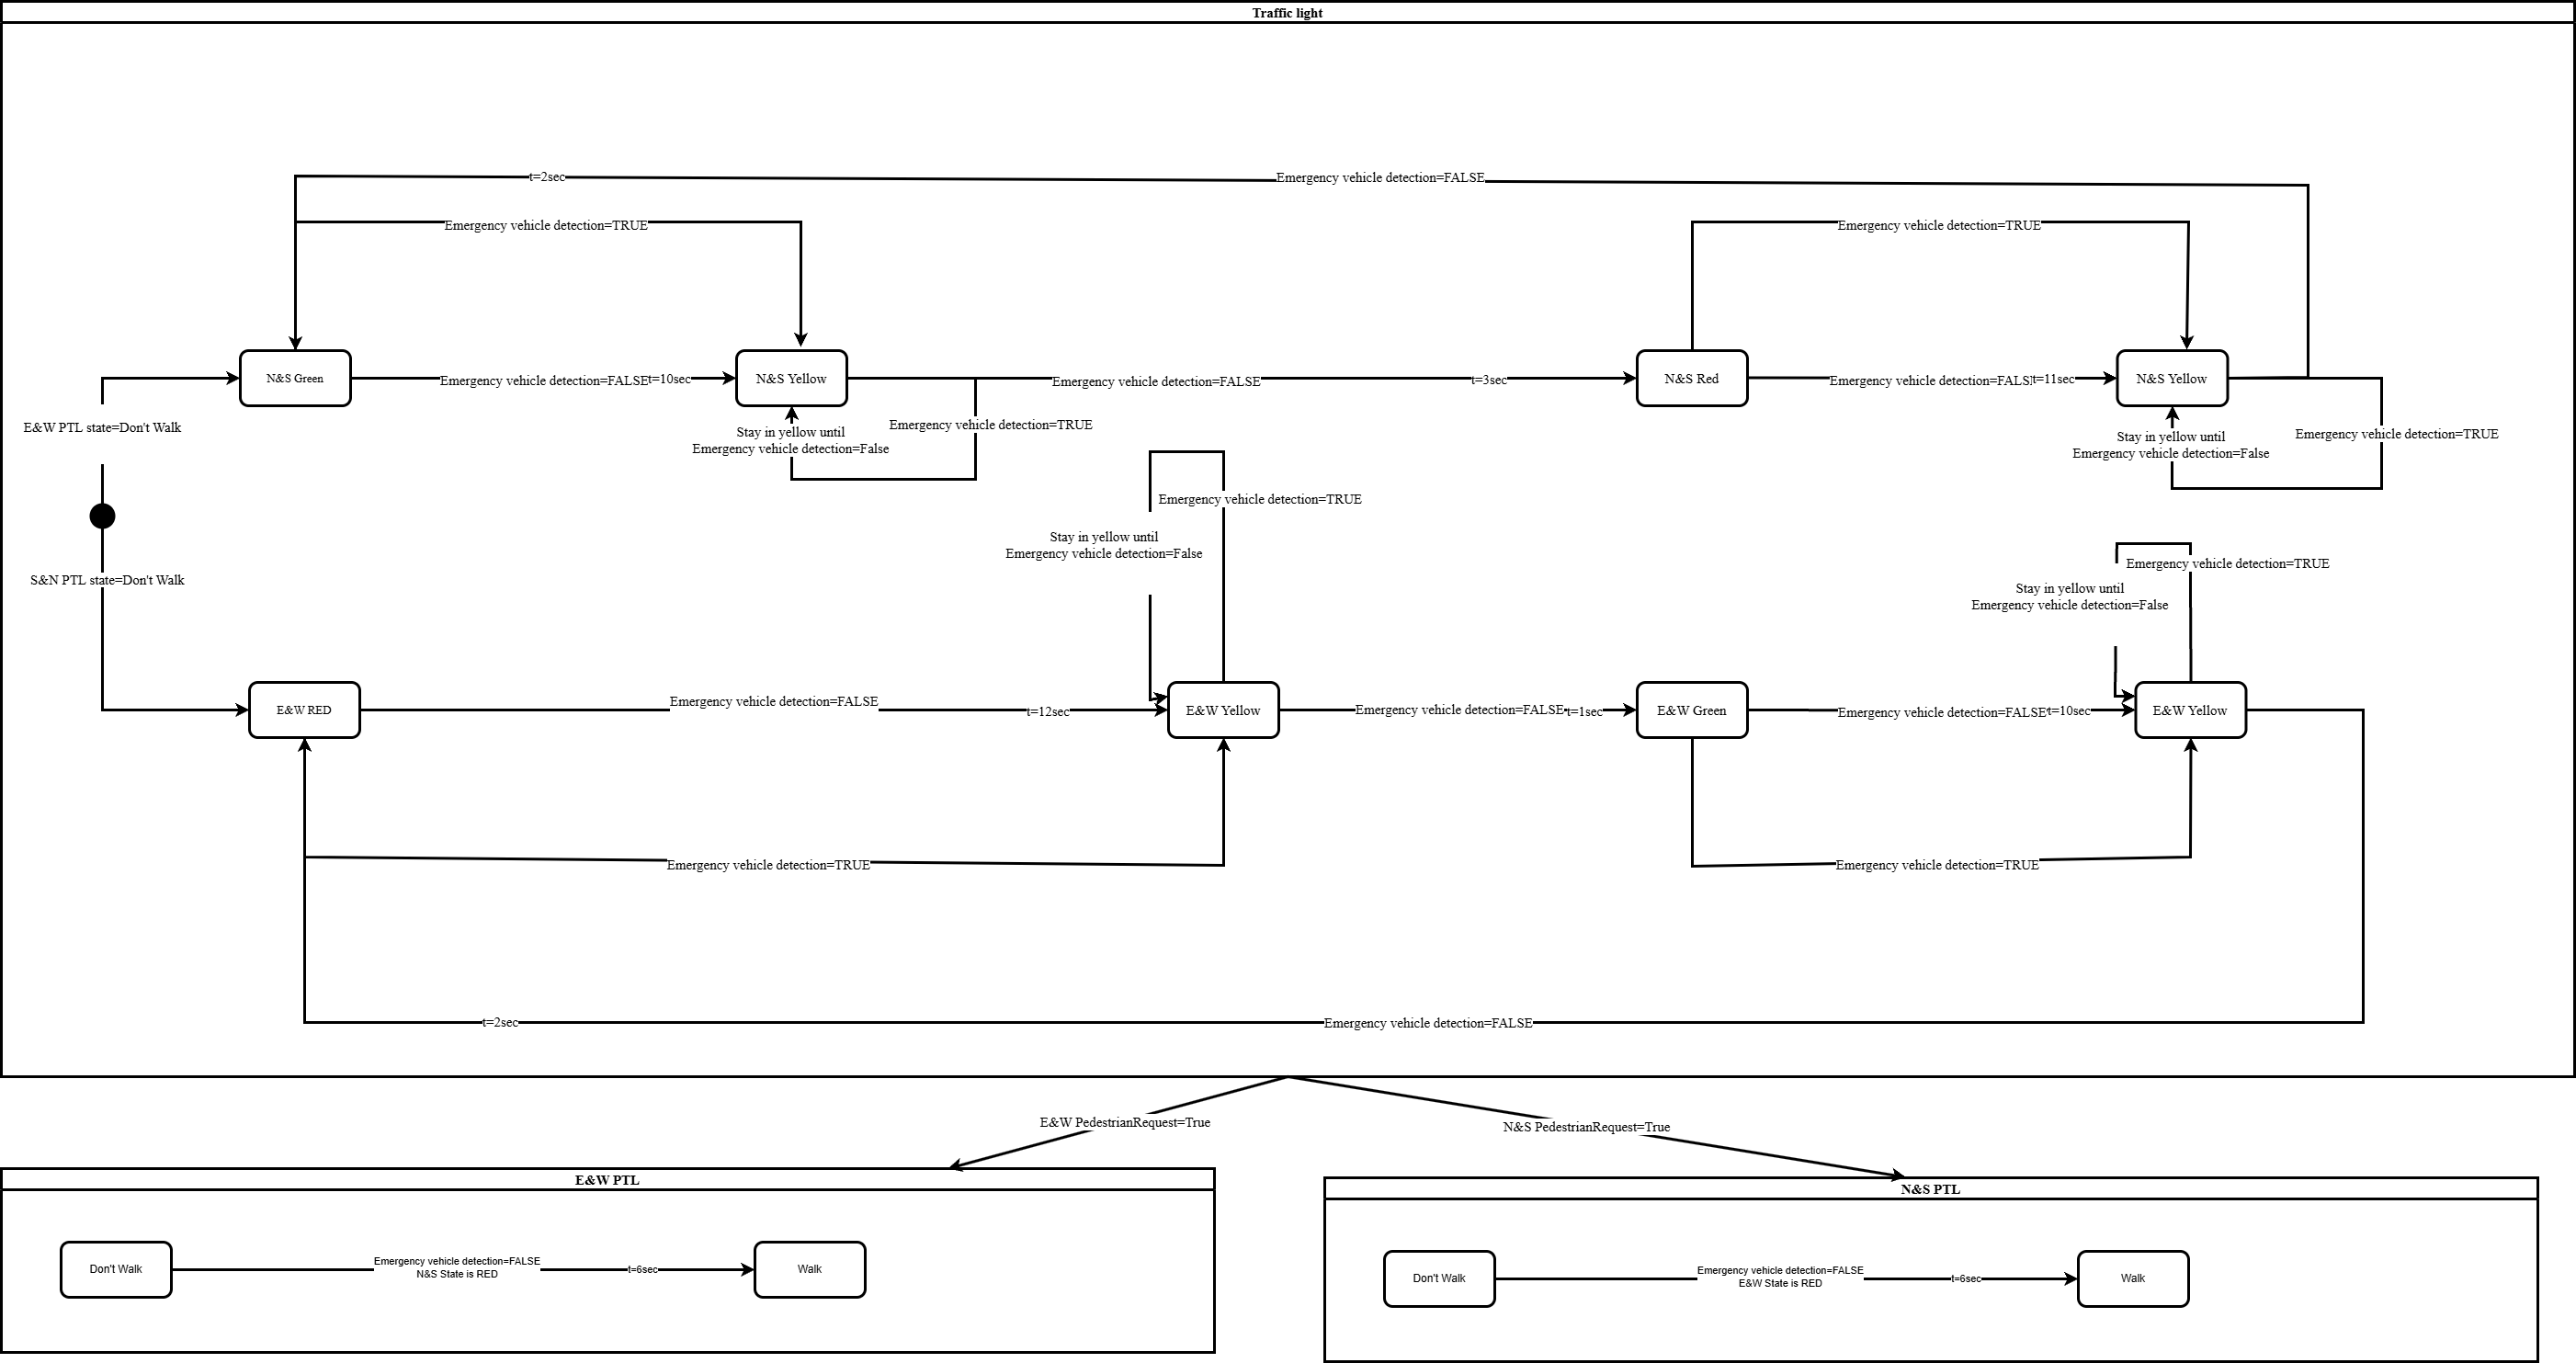
\includegraphics[width=1.0\textwidth]{Pictures/State machine diagram for traffic light and PTL.png}
    \caption{State Machine Diagram}
    \label{fig:state_machine}
\end{figure*}


The behavior of our Traffic Controller is comprehensively modeled using SysML State Machine Diagram that can be seen in Fig. 2. This diagram provides a detailed representation of the system's operational states and the transitions between them, offering insight into the decision-making processes and responses to various stimuli during operation.
The system begins in the "ON" state. From this initial state, the system transitions into the "Idle" state. This state represents the default behavior of autonomous vehicles, where the vehicle is just following the designated path. While in the "Idle" state, the vehicle is continuously monitoring the environment through various sensors, once the sensors detect an intersection, the system transitions into the "Approaching" state. During this state, the vehicle transmits the request to pass the intersection. The traffic controller will check the vehicle position. This decision points to two possible states: "Enter" or "Queued". The choice between these states is determined by the position of the autonomous vehicle in the queue. If the position of the vehicle is not the first, the system will enter the "Queued" state. In this state, the vehicle will wait until it becomes the first in the queue. 
If the corresponding position is the first, the system will proceed to the "Enter" state. During this state, the system will check if the route is safe for the vehicle to proceed without causing any collisions. By doing so, the system will either go into "Wait for car passage" state or "Ready" state. The traffic controller will check: if the previous car is in the way of the next vehicle leading to a collision, the system will go into "Wait for car passage" state. The vehicle will remain in this state until the condition is satisfied and the path is clear. Once safe, the system will move to the "Ready" state. In this current state, the vehicle is ready to exit the intersection, however, in our system pedestrians are given priority, in order for the vehicle to pass, the system has to clear that there are no pedestrians in the designated threshold and the car is able to pass safely. Otherwise, the vehicle will wait in the "Wait for pedestrian to pass" state until the pedestrian has passed safely. Now, the system will transition into the "Cross" state, where the vehicle proceeds through the intersection. Upon completing the crossing, the system reaches the final state, "EXIT", in which the vehicle detaches itself from the traffic control system, allowing the next vehicle to begin its process.
This state machine model captures the dynamic nature of our traffic controller system. It illustrates how the system continuously assesses its environments, makes decisions based on sensors and communication inputs, and adapts its behavior accordingly. The clear definitions of states and transitions ensures the system can handle various scenarios it may encounter leading to optimal coordination, safety, and efficiency in intersection management.


\subsection{Use Case Diagram}


\begin{figure}[h!]
    \centering
    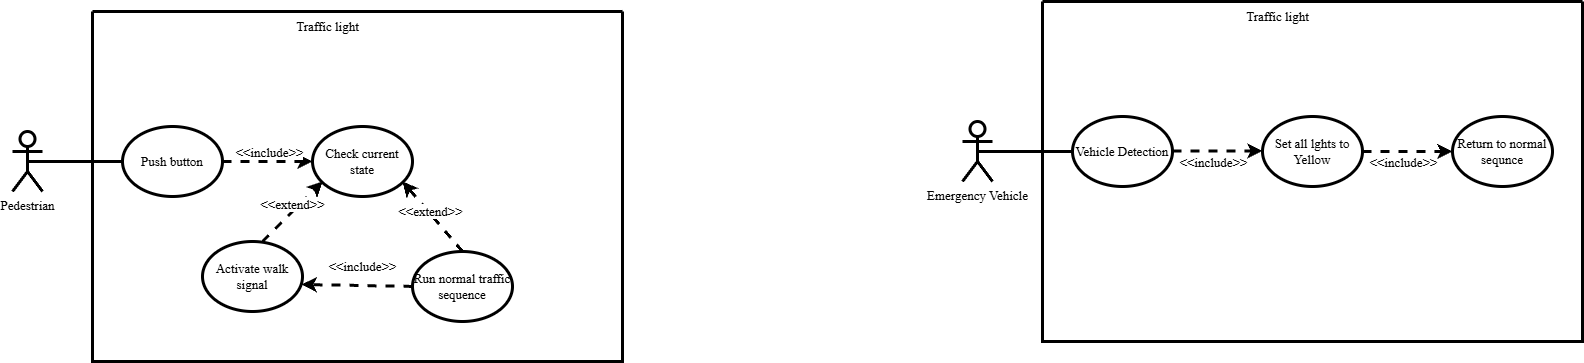
\includegraphics[width=1.0\textwidth]{Pictures/Use_Case_Diagram.png}
    \caption{Use Case Diagram}
    \label{fig:Use Case Diagram}
\end{figure}   

The Use Case Diagram in Fig. \ref{fig:Use Case Diagram} illustrates the interactions between the autonomous vehicle and the traffic controller. The primary actor in this model is the Autonomous Vehicle, which interacts with the controller to navigate the intersection safely. The vehicle initiates the process by sending a request once the vehicle enters the detection range of the controller. This request triggers the controller to check the current queue. If the vehicle is not the first in line, it must wait until it becomes first, that is an extended behavior that is only activated when the vehicle is not the first in the queue meaning this behavior only happen when a this condition is satisfied. Once the vehicle reaches the front of the queue and the path is clear, the system gives permission to pass, allowing the vehicle to safely proceed through the intersection. This diagram effectively captures the communication and decision making processes between the vehicles and the traffic controller.


\subsection{Activity Diagram}
The Activity Diagram for Normal Mode illustrates the procedural flow of the traffic controller system as it manages vehicle movement through an intersection. The process begins when a vehicle approaches the intersection and broadcasts its presence. The system then gathers information about surrounding vehicles to determine its relative position in the queue. If the vehicle is not first, it waits in the queue until its turn arrives. Once it is first in line, the system checks for the presence of pedestrians within the intersection zone. If a pedestrian is detected, the vehicle remains in a waiting state until the pedestrian has safely passed. When the path is clear, the vehicle proceeds to cross the intersection and, upon completion, exits the system, allowing the next vehicle to be processed. This diagram effectively captures the logical flow and decision making steps that ensure safe and coordinated traffic movement.
\begin{figure*}[t]
    \centering
    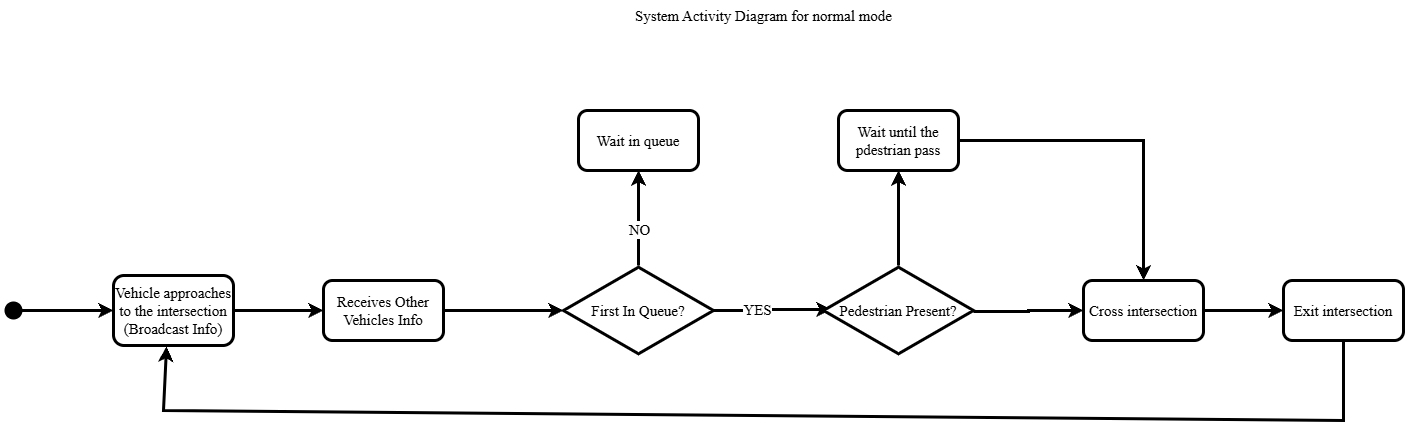
\includegraphics[width=1.0\textwidth]{Pictures/Sys_Activity_Diagram_for_Normal_Mode.png}
    \caption{Activity Diagram for normal mode}
    \label{fig:Activity Diagram}
\end{figure*}

\section{UPPAAL Modelling for deadlock verification}
Traditional traffic intersections use traffic lights to regulate flow. This simulation explores an alternative system: one where cars communicate with each other and with pedestrian indicators to navigate intersections safely. Using UPPAAL, we model timed automata for cars and pedestrians to show how such a system can work. The intersection has four sides—North, South, East, and West—and all sides follow the same behavior. For simplicity, the South side is used to describe the core logic.
\subsection{Intersection Lane Structure and Car Templates}
Each side of the intersection has three lanes: left, middle, and right. The left lane is primarily for incoming traffic and is not used actively in this simulation. The simulation focuses on two templates from the South side:


\begin{itemize}
    \item \texttt{CarSM (Car South Middle)}
    \item \texttt{CarSR (Car South Right)} \\
\end{itemize}


Each car template includes states such as \textit{Arrived}, \textit{ZebraCrossing}, \textit{GoStraight}, \textit{LeftTurn}, \textit{Stop}, and \textit{Moving}.

\begin{figure}
    \centering
    \includegraphics[width=1\linewidth]{Screenshot 2025-07-05 213352.png}
    \caption{Pedestrian on North-South Facing On West}
    \label{fig:enter-label}
\end{figure}


\subsection{CarSM Behavior}
When a car enters via the South middle lane (CarSM), it checks if a pedestrian is crossing the South zebra crossing. If a pedestrian is crossing, it waits. If not, it moves on. The car then randomly decides whether to go straight (toward North) or turn left (toward West). If it turns, it stops again at the West crossing and checks for pedestrians before moving.

\subsection{CarSR Behavior}
The South right lane (CarSR) car always turns right toward East. It first checks the South crossing for pedestrians. After that, it stops again at the East crossing and only continues if no pedestrian is crossing. This flow ensures safe interaction between cars and pedestrians.
\begin{figure*}
    \centering
    \includegraphics[width=1\linewidth]{Screenshot 2025-07-05 212806.png}
    \caption{Model for Cars on Middle Lane of South}
    \label{fig:enter-label}
\end{figure*}

\begin{figure*}
    \centering
    \includegraphics[width=1\linewidth]{Screenshot 2025-07-05 213249.png}
    \caption{Model for Cars on Right Side of South}
    \label{fig:enter-label}
\end{figure*}


\subsection{Pedestrian Modeling}

There are four pedestrian templates in the model:
\\
\begin{itemize}
    \item \texttt{PedestrianNorthSouthFacingOnWest}
    \item \texttt{PedestrianEastWestFacingOnNorth}
    \item \texttt{PedestrianEastWestFacingOnSouth}
    \item \texttt{PedestrianNorthSouthFacingOnEast}\\
\end{itemize}
Each pedestrian automaton has two states:
\begin{itemize}
    \item \texttt{Crossing}
    \item \texttt{Crossed}
\end{itemize}
A global timer is implemented via a separate template called \texttt{Ticker}, which controls when each pedestrian begins and ends crossing.

The crossing durations are as follows:
\begin{itemize}
    \item South pedestrians: 10 time units
    \item East pedestrians: 7 time units
    \item West pedestrians: 3 time units
    \item North pedestrians: 14 time units
\end{itemize}

When a pedestrian starts crossing, it emits a synchronization signal such as:
\begin{center}
    \texttt{PedestrianOnSouthCrossing!}
\end{center}

After the crossing is complete, it emits another signal:
\begin{center}
    \texttt{PedestrianOnSouthCrossed!}
\end{center}

These synchronization channels are used by car templates to decide whether to wait or proceed, based on pedestrian activity at the crossings.

\subsection{System Integration}

The system ties all templates together using synchronization channels and guards. There are no random clocks; all timing is deterministic through the globalTime and anotherglobalTime counters. All car templates (CarSM, CarSR, etc.) and pedestrian templates are declared in the system block and simulate real-time movement across the intersection.

\section{Hardware-Software Co-Design Implementation}
The purpose of this section is to discuss the hardware-software co-design part of the implementation. Therefore, obviously the section are divided into two parts: FreeRTOS (Software) in subsection \ref{subsec: FreeRTOS} and Hardware Realisation in \ref{subsec: hardware}. 
\subsection{FreeRTOS}
\label{subsec: FreeRTOS}
To realize the system in a simulation format with real-time capabilties, we employed a real time operating system (RTOS), in this case the open-source FreeRTOS library. In FreeRTOS, just like in real systems, functions that have to meet a deadline are called tasks. Therefore, to realize a working simulation, we created many critical tasks. This section focuses on some of these important tasks and our solution to resolving conflicts at critical parts of the system. 

\subsubsection{vCarGeneratorTask()}
This task is responsible for the safe spawning of cars from any of the four lanes. It employs efficient error handling to make sure cars are properly allocated and initialized. A state machine diagram illustrating the flow of this task can be seen in \ref{fig:car-gen-sm}. 

\begin{figure}[h!]
  \centering
  \includegraphics[width=0.5\textwidth]{carGeneratorTask.png}
  \caption{State machine for Car generator task}
  \label{fig:car-gen-sm}
\end{figure}


\subsubsection{vCarTask()}
After the cars have been generated, the Car structure with parameters as seen in fig. \ref{fig:carStruct} is activated. In this task, all varaibles in the struct are initialized. Every action of the car from entering the simulation area, to reaching the critical section, to exiting the simulation is covered in this task and is logged accordingly. Important FreeRTOS features like queues for efficiently inter-task messaging and semaphores to ensure efficient resource sharing of the scheduler time are used as well. A state machine diagram detailing the flow of the task can be seen in fig. \ref{fig:carGnerator}.

\begin{figure}[h!]
    \centering
    \includegraphics[width=0.6\linewidth]{carStruct.png}
    \caption{Class Diagram showing the Car struct}
    \label{fig:carStruct}
\end{figure}

\begin{figure}[h!]
  \centering
  \includegraphics[width=0.5\textwidth]{carTask.png}
  \caption{State machine for Car generator task}
  \label{fig:carGnerator}
\end{figure}


\subsubsection{log\_\_event()}
To visualize the system using the pygame library in Python, it was important to efficiently log all actions of the car from the earlier discussed car task. This task was in charge of this function and creating a CSV log file whose contents were parsed into a Python script to visualize our system.

\subsubsection{Conflicts at critical section}
It was important to define what part of this system are susceptible to collisions. We call this the critical section. In this case, we define the Intersection as the critical section, because it is a meeting point for all the cars coming from different lanes. There are different approaches to solving this conflict. We decided to use a First Come First Serve (FCFS) algorithm. While seemingly trivial, it ensures proper queuing and ensures fairness for all cars in the system.

To implement this in our FreeRTOS system, we created an Arbiter task (varbiterTask()). The main responsibility of this task was to "peek" at the head of all four queues, check for the car with the earliest arrival time and release (through a mutual exclusive binary semaphore) that car and only that car to the Intersection.  This approach ensures smooth scheduling of the cars and prevents collisions. 
The sequence of operations can be seen in \ref{fig:arbiter-seq}.

\begin{figure}[h!]
  \centering
  \includegraphics[width=0.5\textwidth]{seqDiagram.png}
  \caption{Sequence diagram for Car generator task}
  \label{fig:arbiter-seq}
\end{figure}

\subsection{Hardware Realisation}
\label{subsec: hardware}
As traffic control systems require deterministic behaviour, the arbiter logic is realised in hardware. Additionally, the inputs to the arbiter are also realised in a separate hardware module called requesting detection. This is discussed in subsection \ref{subsec:arbiter} and \ref{subsec:reqdetc}.
\subsubsection{Vehicle Arbiter Module}
\label{subsec:arbiter}
The arbiter controls traffic flow from four directions (North, East, South, and West) by granting access to one direction at a time, based on a simple state machine. It rotates access to each direction in a round-robin fashion , regardless of whether a vehicle is actually waiting. On every rising clock edge, the state rotates to the next one. It doesn’t check if a car is waiting as it blindly cycles. Each grant signal is 1 only when the machine state matches that of the request signal resulting in fair rotation. This is designed in VHDL and the block diagram is generated in Vivado as shown in fig, \ref{fig:arbiter module}.

\begin{figure*}
  \centering
  \includegraphics[width=1\textwidth]{Arbiter.png}
  \caption{Schematic for Arbiter Module}
  \label{fig:arbiter module}
\end{figure*}

\subsubsection{Request Detection Logic}
\label{subsec:reqdetc}
The RequestDetector is designed to monitor the presence of vehicles at each road (North, East, South, West) and generate request signals so that the arbiter can use to decide who should get access. This would typically come from sensors that detect cars approaching the intersection. On each rising edge of the clock the request signal is copied directly from the sensor signal. If a sensor detects a vehicle ,for example, sense\_N = '1', then req\_N becomes '1'. The schematic can be seen in fig. \ref{fig:req}.
\begin{figure}[h!]
    \centering
    \includegraphics[width=1\linewidth]{Request Detector.png}
    \caption{Module modelling a sensor to detect cars approaching.}
    \label{fig:req}
\end{figure}



\section{Outcome}
Several challenges were faced in mapping from model created in UPPAAL to FreeRTOS implementation. Because of this some cars were stuck in deadlocks. This led to changing the final development from 3 lanes per road to 2 lanes per road as shown in fig. \ref{fig:final output}. The complete documentation can be found in \url{https://github.com/RubayetKamal/SS2025_Embedded_Electronic_Enginering_A_Lab_Team1}
\begin{figure}[h!]
    \centering
    \includegraphics[width=1\linewidth]{FinalOutput.png}
    \caption{Output Visualised.}
    \label{fig:final output}
\end{figure}



\section{Conclusion}
In this paper, a centralized, real-time cross-traffic management system tailored for autonomous vehicles at intersections is presented. Motivated by the disadvantages of traditional traffic light systems, centralized controller is implemented that enforces a First-Come, First-Serve (FCFS) queuing mechanism while prioritizing pedestrian safety. Using SysML and UPPAAL, system behavior has been modelled and verified deadlock-free execution. Implementation was realized through hardware-software co-design, utilizing FreeRTOS for real-time task scheduling and VHDL for deterministic arbitration. Despite the success of the system, several challenges were encountered, particularly in aligning the UPPAAL model with the FreeRTOS task structure, which led to simplifications in lane design. 

The system demonstrates effective and safe traffic coordination for autonomous vehicles in simulation. For future work, the proposall is on extending the system to handle dynamic prioritization (e.g., emergency vehicles), supporting more complex intersection layouts, and integrating machine learning techniques for predictive traffic flow optimization. Moreover, a full-scale hardware prototype can be developed and tested in a physical environment to validate the robustness and scalability of the approach.

\section*{Acknowledgment}
This project has been possible due to the constant feedback of Prof. Dr. Henkler throughout the course. His expertise and guidance of FreeRTOS contributed to completion of the project.



\begin{thebibliography}{00}
\bibitem{vivado}
Vivado Design Suite, Xilinx Inc. [Online]. Available: \url{https://www.xilinx.com/products/design-tools/vivado.html}
\bibitem{modelsim}
ModelSim Simulation Tool, Mentor Graphics. [Online]. Available: \url{https://www.mentor.com/products/fv/modelsim/}
\bibitem{freertos}
FreeRTOS Real-Time Operating System, Real Time Engineers Ltd. [Online]. Available: \url{https://www.freertos.org}

\end{thebibliography}

\end{document}
